\chapter{Experiments}\label{experiments}
To complete the last research task proposed in the introduction \hyperref[problem_definition]{T4}, collected datasets are leveraged to built a media bias classifier which is subsequently used for inference over Czech News data. 

Architecture-wise, a pre-trained transformer language model (\ref{att_transformers}) is used. The reviewed models were pre-trained solely on Czech data or on multiple languages jointly. A classifier consisting of a dense\footnote{Often referred to as fully-connected layer.} layer is attached to the language model output to perform the binary classification task. The scheme of the particular architecture used can be seen in \ref{fig:classifier}.


Despite the fact that there were eight other datasets collected, the final classifier is \textbf{fine-tuned} (and evaluated) only on the BABE dataset due to its high quality and properties. All other datasets serve as an auxiliary data only.

In this context, \textbf{fine-tuning} is essentially a process of adapting the language model and the classification head to the BABE dataset. Both the parameters of the language model, e.g. BERT, and the parameters of the classifier are updated jointly. The weights of the classification layer are trained from scratch; on the other hand, the pre-trained language model already contains meaningful linguistic features, so in the process, its parameters are \textbf{fine-tuned} for bias-specific representations. This is especially convenient since the BABE dataset has only about 3700 sentences. Therefore, training from scratch would likely fail to learn general linguistic properties together with subtle bias features.






\begin{figure}
\makebox[\textwidth][c]{
  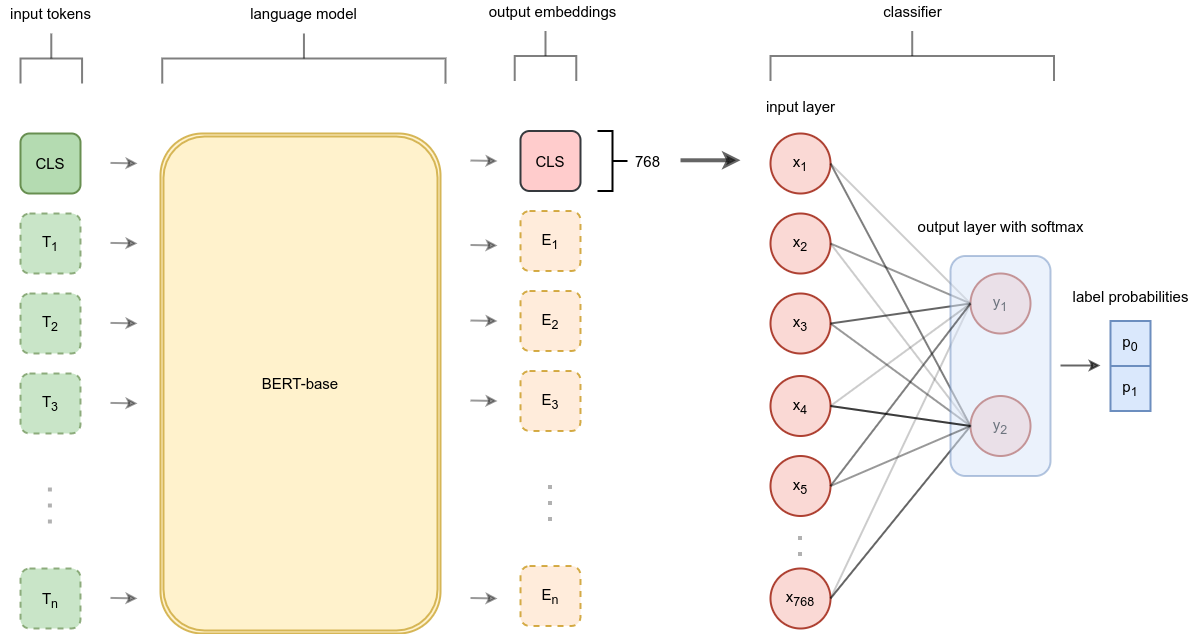
\includegraphics[scale=0.3]{my_modules/multimedia/final_colored.png}
  \caption{Scheme of a text classification architecture used in the fine-tuning process.}
  \label{fig:classifier}
  }
\end{figure}


Morover, the effects of further \textbf{pre-training} are studied to answer the two main research questions, \hyperref[Q1]{Q1} and \hyperref[Q2]{Q2}. This means that before fine-tuning on BABE, the language model with the classifier is further pre-trained on a combination of auxiliary bias datasets. The purpose of secondary\footnote{Primary pre-training is the original unsupervised pre-training task executed by the authors of the particualr language model.} pre-training is to learn subtle \textbf{bias representations} and therefore help with subsequent fine-tuning on the BABE.

A Scheme of the whole process pipeline can be seen in figure [fig].

Because of novelty of the CWNC I also perform a baseline fine-tuning and evaluation on this dataset, no further experiments are carried out on CWNC.

As opposed to English language, there is a relatively low number of Czech pre-trained transformer models available. A list and a brief summary of all the models tested in the experiments can be found in the following:




\subsection{Czech monolingual models}
Models trained solely on Czech data.
\begin{itemize}
    \item \textbf{RobeCzech} \cite{strakarobeczech} - RoBERTa-based model with 125M parameters. Like its original counterpart, it is trained with the \gls{mlm} task, on 4,917M tokens of Czech corpora.
    \item \textbf{Czert} \cite{sido-etal-2021-czert} - BERT-based model with 110M parameters, trained with \gls{nsp} tasks. All Together trained on 37GB of text. 
    \item \textbf{FERNET-C5} \cite{lehevcka2021comparison} - BERT-based model trained with the \gls{mlm} and \gls{nsp} task on 93GB of text from the Common Crawl project.
    \item \textbf{FERNET-News} \cite{lehevcka2021comparison} - RoBERTa-based model trained with \gls{mlm} task on 20GB of Czech News text.
\end{itemize}




\subsection{Multi-lingual models}
Models trained jointly on multiple languages.
\begin{itemize}
    \item \textbf{SlavicBert} \cite{arkhipov2019tuning} - BERT-based model with 179M parameters, trained on four languages: Russian, Bulgarian, Czech, and Polish. The model is trained on all 4 languages at once. The model is not trained from scratch, but it is a fine-tuned version of mBERT.
    \item \textbf{mBERT} \cite{devlin2019bert} - BERT-based model with 179M parameters trained on corpora of 104 languages, including Czech, with MLM task.
\end{itemize}




\section{Experimental setup}
All models are fetched, trained, and evaluated using the HuggingFace API\footnote{\url{https://huggingface.co/docs}}. The maximum sequence length is set to 128 tokens. All parameters can be seen in the Appendix \ref{all_parameters}.

A small portion (15\%) of the target dataset is left aside as a \textbf{test set} at the beginning and is used only for the final evaluation to ensure that no test data leak into the training data.

Every fine-tuning, except the one performed on the final test set, is evaluated using a 10-fold \gls{cv}. This helps to get more realistic estimates of model performance than a simple train-validation split would give. The only evaluation metric used for all experiments is the F1 score with \textit{macro} averaging\footnote{The F1 score is computed for both classes and averaged.}. 

All training has been done on the RCI cluster node with 4 x NVIDIA Tesla V100 with 32GB GPU graphic memory.





 \section{Baseline setup}
 As a baseline, all Czech and multilingual models are fine-tuned on BABE and evaluated using a 10-fold stratified \gls{cv}. The hyperparameters used are the same as those used by the authors of BABE \cite{Spinde2021MBIC}. However, the authors used early stopping together with \gls{cv} and used the validation split inside \gls{cv} to early stop. This allows the model to "see" the test data during the training. This condition may lead to too optimistic results.
 
 A solution to this problem would require another split for validation, but at this point, the size of the training data is already shrunk significantly. Therefore, I did not use the early stopping together with \gls{cv} at all. Instead, I fixed the number of epochs to 3 as suggested by the authors of BERT \cite{devlin2019bert} . 
 All other hyperaparemeters remained unchanged; AdamW optimizer is used with an initial learning rate of 5e-5 and a batch size of 64.
 
 The baseline evaluation of all Czech models used can be seen in table \ref{table:3}. The final F1 score is averaged across all folds.
 
 The model that performs best on the BABE is \textbf{FERNET-C5}. It also performs best on the novel CWNC dataset; therefore, it is a suitable candidate for further tuning. From now on, all experiments are performed using this model.
 

 \begin{table}
\makebox[\textwidth][c]{
\begin{ctucolortab}
\begin{tabular}{c||c|c|c|c|c|c}
 \textbf{target}\textbackslash \textbf{models} & \textbf{Czert} & \textbf{RobeCzech} & \textbf{mBERT} & \textbf{FERNET-C5} & \textbf{FERNET-News} & \textbf{SlavicBERT}\\
 \hline
 \hline
 \textbf{BABE} & 0.739 & 0.773 & 0.743 & \textbf{0.78} & 0.644 & 0.762 \\
 \hline
 \textbf{CWNC} & 0.726 & \textbf{0.758} & 0.734 & 0.689 & 0.602 & 0.729 \\
\end{tabular}
\end{ctucolortab}
\caption{F1 scores of baseline fine-tuning. Best scores for each dataset are highlighted.}
\label{table:3}
}
\end{table}

 
 
 
 
\newpage

 \section{Hyperparameter tuning}
I restricted the search space of hyperparameters only to the combinations of:
 \begin{itemize}
     \item \textbf{Batch size} $\in \{16,32\}$
     \item \textbf{Learning rate} $\in $ \{2e-5,3e-5,5e-5\}
     \item \textbf{Epochs} $\in \{2,3,4\}$
 \end{itemize}
 
 As the authors of the original BERT paper suggest. Then I ran a grid search with \gls{cv}. The overall best parameters were as follows:
 \begin{center}
      \{learning\_rate = 3e-5,batch\_size = 32, epochs=3\}\label{hyperparams}
 \end{center}
 
 The model with the best parameters achieved a 0.784 F1 score ($\sim$0.4\% improvement against baseline).


 
 
\begin{table}
\makebox[\textwidth][c]{
\begin{ctucolortab}
\begin{tabular}{c||c|c|c|c|c|c|}
  & \textbf{baseline} & \textbf{SUBJ} & \textbf{WIKI} & \textbf{MB} & \textbf{WNC} & \textbf{ALL}\\
 \hline
 \hline
 \textbf{Pretraining + Finetuning} & 0.7835 & 0.7875 & 0.7797 & 0.7702 & 0.7825 & \textbf{0.7878} \\
 \hline
 \textbf{Pretraining + Evaluating} & - & 0.5542 & 0.6344 & 0.4631 & \textbf{0.6697} & 0.6423 \\
\end{tabular}
\end{ctucolortab}
\caption{F1 scores of effects of pretraining on different dataset combinations.}
\label{table:4}
}
\end{table}





\section{Combining Datasets}
This section is dedicated to the study of the influence of pre-training on combinations of datasets. Trying all combinations would result in training 255 models\footnote{Given a set of $n$ elements, number of subsets is $2^n$. Here, we have a set of eight datasets, resulting in 256 subsets. 255 without an empty set.}, which is infeasible for obvious reasons. Therefore, I decided to experiment with pre-training on five subsets of datasets with regard to their bias information, to see which of them can serve as a good initialization for fine-tuning on BABE.
The combination sets are as follows:
\begin{itemize}
    \item \textbf{SUBJe} - is a combination of SUBJ and MPQA dataset, which both focus on explicit subjective bias.
    \item \textbf{MB} - is a combination of NJNJ, UA-crisis and BASIL dataset which are all from the \gls{mb} family.
    \item \textbf{WIKI} - are all datasets collected from Wikipedia. It consists of CW-hard, WikiBias, and CWNC. The three datasets were collected automatically with respect to NPOV violations as described in \ref{wiki-npov}.
    \item \textbf{ALL} - This one is simply a combination of all datasets except the WNC.
    \item \textbf{WNC} - WNC is almost 90\% of all data; therefore, I perform experiments on this dataset separately.
\end{itemize}
 
In every combination, the data were randomly mixed and subsequently downsampled, so that classes were balanced. For each combination, 20\% of data were used as a validation set to decide the optimal number of epochs for pre-training. The convergence of validation losses can be seen in the figure \ref{fig:all_losses}. The number of epochs for pretraining were chosen as follows: 1, 3, 1, 2, 1 for SUBJe, MB, WIKI, ALL and WNC respectively.
\begin{figure}
  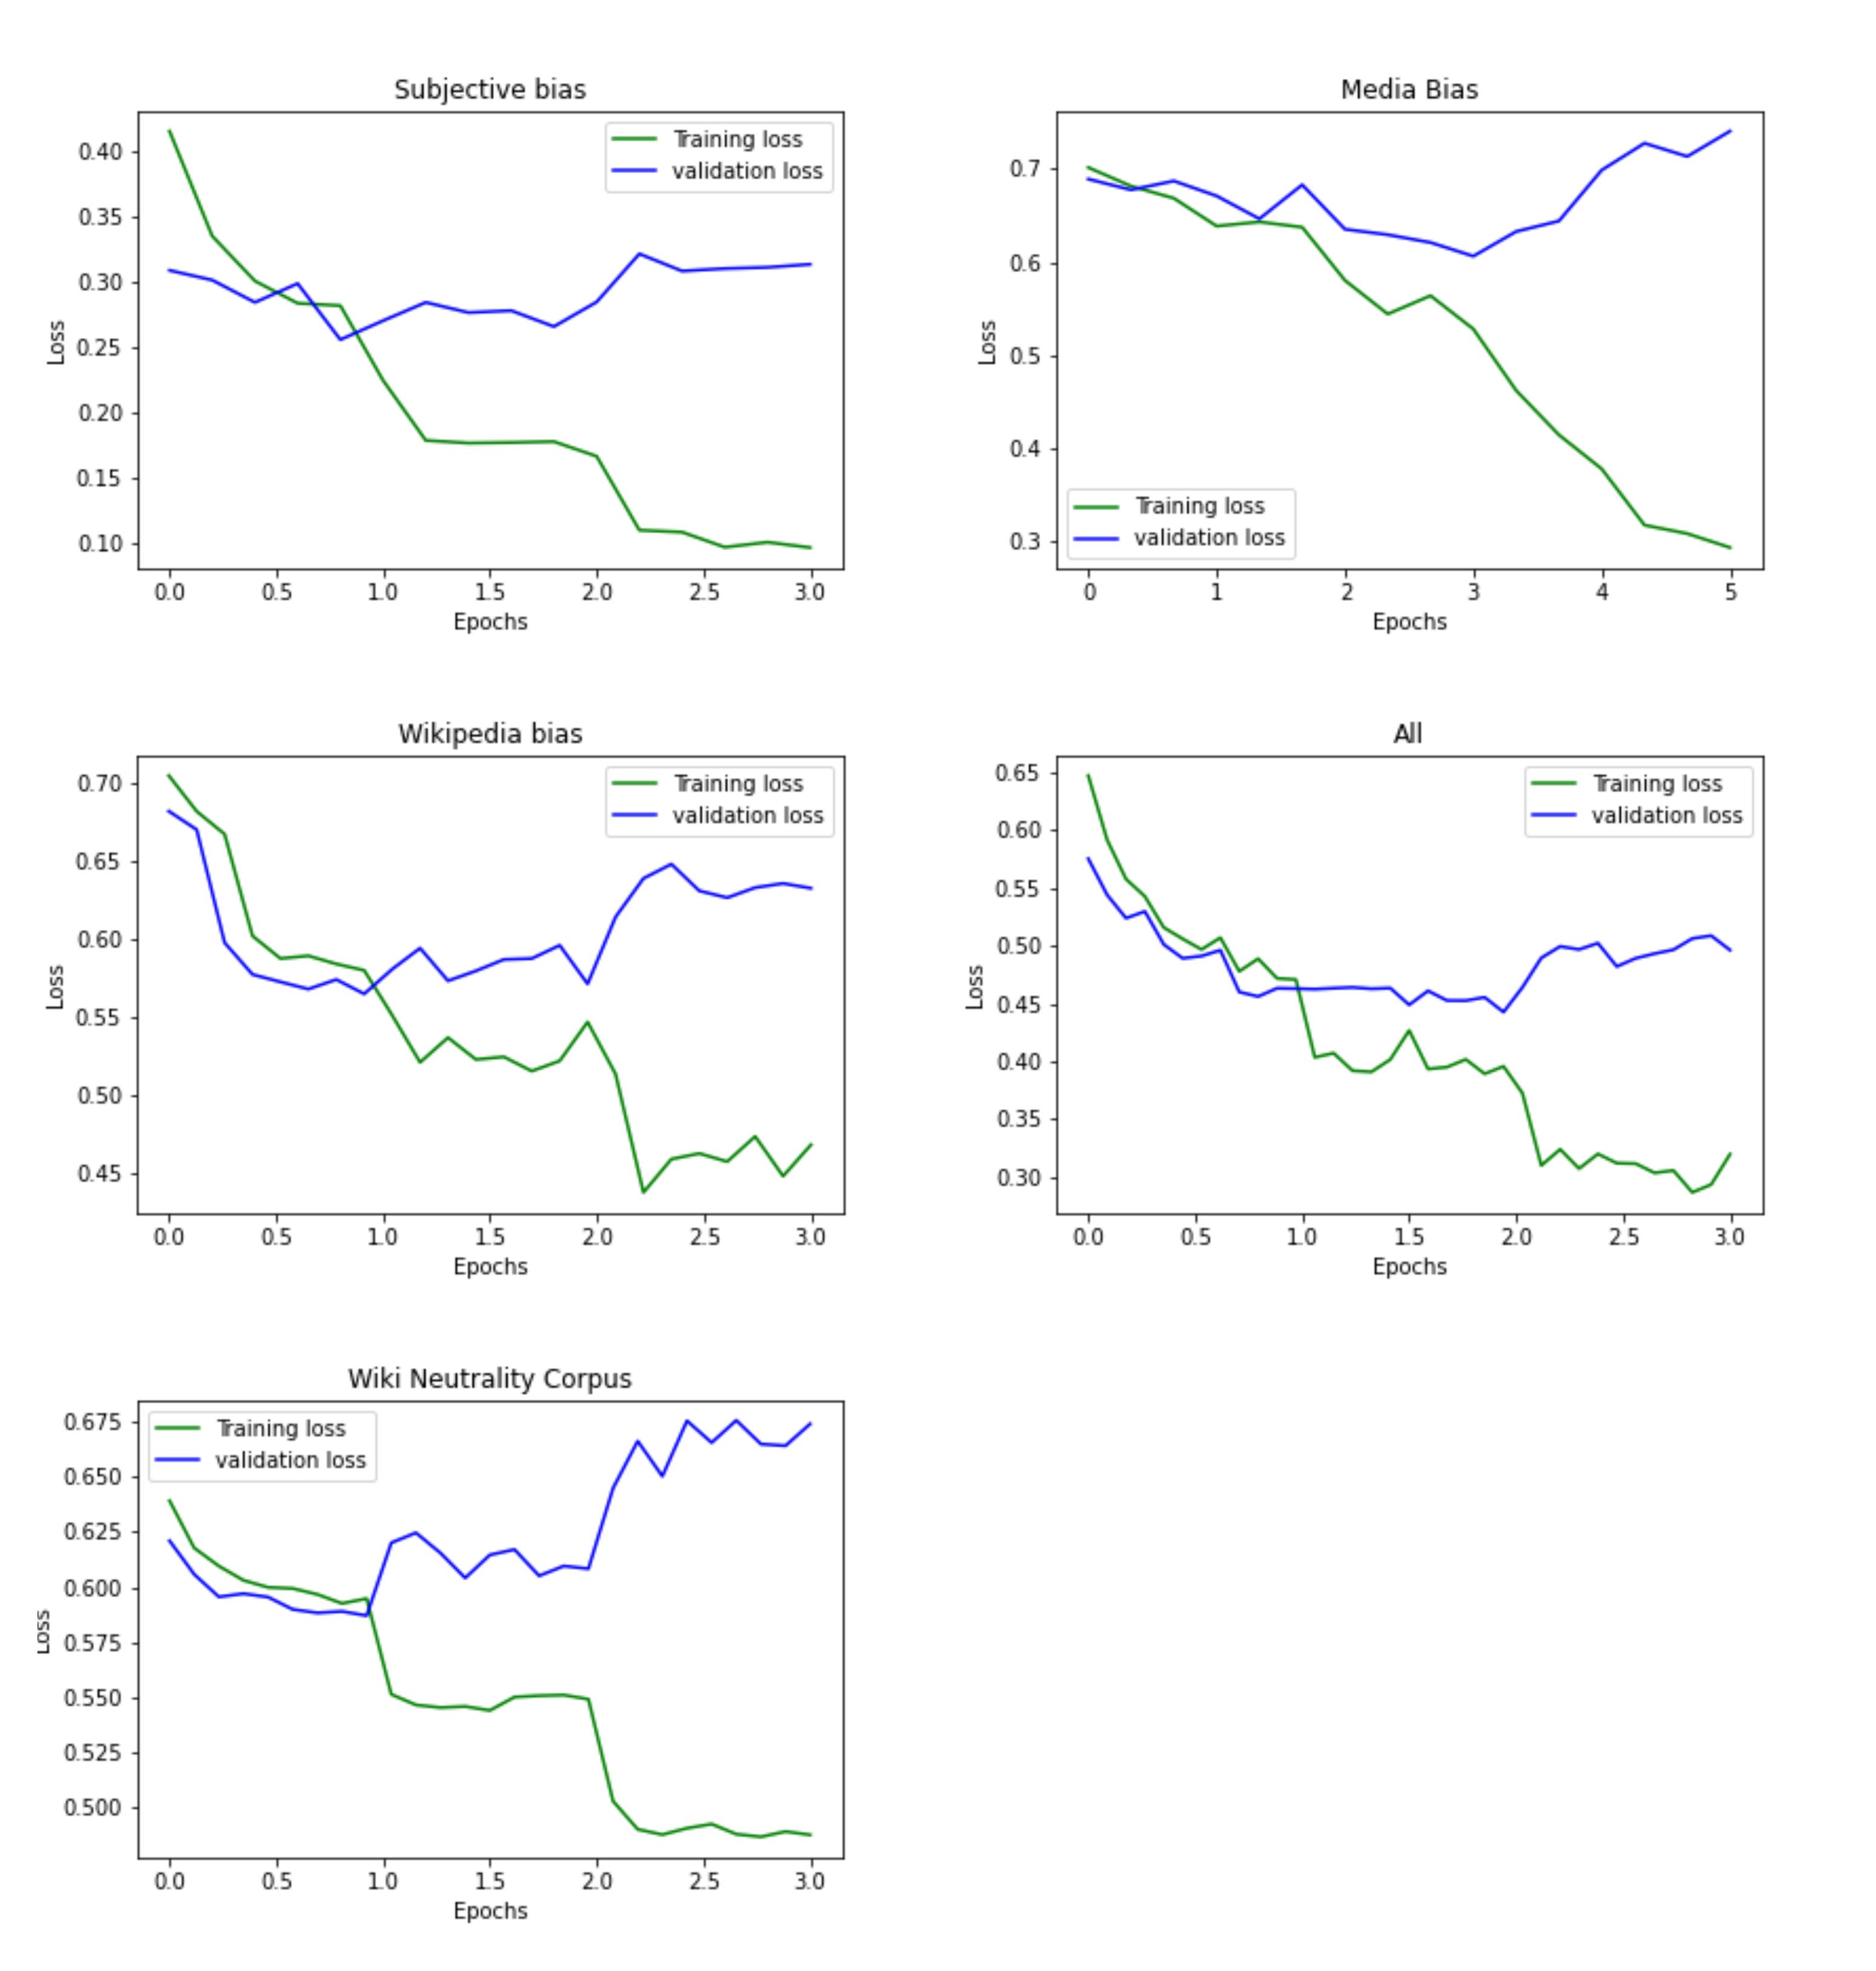
\includegraphics[scale=0.5]{my_modules/multimedia/all_losses.png}
  \caption{Convergence of validation loss over different dataset combinations}
  \label{fig:all_losses}
\end{figure}


\subsection{Pre-training + Evaluating}
To answer the question \hyperref[Q1]{Q1}, the models pre-trained on the combinations of bias datasets are evaluated in BABE without fine-tuning it. This way, it can be studied how well each model trained on each set can transfer knowledge to the detection of \gls{mb} in BABE. Thus, possibly unveils the relatedness to BABE. The results can be seen in table \ref{table:4}. In the table, this pre-training \textbf{without} further fine-tuning is referred to as \textbf{Pre-trained}.

There is clear evidence that models pre-trained on Wikipedia data, both \textbf{WIKI} and \textbf{WNC} perform relatively well compared to \textbf{MB} and \textbf{SUBJ}. This suggests that the bias distribution in WIKI datasets is the closest to BABE.

During pre-training, the F1 score of the WIKI and the MB set both peaked around 70\% on their validation sets; however, the model trained on MB generalized very poorly to BABE data as opposed to the WIKI model (0.46 against 0.67). I suspect that this result is due to the high size imbalance between the two sets.

In conclusion, models that generalize to BABE the best are pre-trained on Wikipedia NPOV data.

\subsection{Pre-training + Fine-tuning}
Secondly, pre-trained models are used as a sort of weight initialization for fine-tuning on the BABE. The results can be seen in table \ref{table:4}. This process is referred to as \textbf{Pre-trained + Fine-tuned}.

Pre-training on \textbf{ALL} datasets combined resulted in the best performance; however, virtually the same performance was achieved by the model trained on the \textbf{SUBJe} combination. The difference is statistically insignificant. Importantly, the SUBJ split represents almost half of all data (see \ref{fig:cz_data}). Therefore, I assume that the performance of ALL split is high because of the presence of SUBJe.

Pre-training on the other sets hurts the performance. Yet, the difference is very small. The lowest score is achieved by pre-training on MB set. I suspect this is mainly due to the small size (2500 sentences) of the balanced MB set that may have led to overfitting.

In conclusion, pre-training on subjective bias datasets helped with \gls{mb} detection in BABE.




\section{Results}
The final FERNET-C5 model has been pre-trained with \textbf{ALL} datasets combination and fine-tuned with the optimal parameters (\ref{hyperparams}) on BABE target dataset. Finally, on a \textbf{test} set it achieved an F1 score of \textbf{0.804}.

Subsequently, for the final model that I share\footnote{\url{https://huggingface.co/horychtom/czech_media_bias_classifier}} on huggingface and which is used for inference experiments, the entire BABE dataset, including the test set, is used for training.

\section{Discussion}
The results suggest that subjectivity bias as opposed to media bias appears to be a bit more explicit and straightforward, since pre-training on the subjectivity task helped with \gls{mb} detection, but proved insufficient without further fine-tuning (only 55\% on BABE). This supports the assumption that \gls{mb} is composed of many more superficial linguistic features \ref{features}.

Also, despite the relatively high performance, the final score on the test set is not representative due to its size. The test set consists of $\sim$ 500 sentences and therefore, may not adequately represent all bias information. For a better evaluation, I propose using a nested \gls{cv}.

The authors of the original paper that introduces BABE \cite{spinde2021neural} report an F1 score of $\sim$ 0.8 for fine-tuned transformer model. That is approximately 2\% higher score than I achieved on the Czech version. This may be caused either by the noise introduced into the data during machine translation, or by the possibly lower quality of the Czech pre-trained models.

Prehaps, a complete study with more models could be performed, but that would require an enormous number of trained models. Essentially, these results show that there was a minimal gain over the baseline (\textbf{+0.7\%}).

The results indicate that the overall low quality and limited size of the available datasets make their use for media bias detection impractical.







\newpage

\section{Inference on Czech News Samples}\label{inference}

\begin{itemize}
    \item abstract,headline, text bias correlation
    \item vbias progress over time for one domain
    \item plot the difference between domains
    \item plot the difference between topics
    \item info about 'commentary' articles is presented! super
\end{itemize}

vhodný články
\begin{enumerate}
    \item \url{https://www.novinky.cz/domaci/clanek/jak-cist-volby-294694}
    \item tahle je asi nej ta pod timhle
    \item \url{https://www.novinky.cz/zahranicni/evropa/150611-v-rakouskych-volbach-podle-pruzkumu-triumfuji-pravicovi-populiste.html}
\end{enumerate}

\subsection{Demo}
Additionally, I provide a simple web demo for the reader to experiment with\footnote{\url{https://huggingface.co/spaces/horychtom/czech_media_bias_detection}}. The use of the demo can be seen in \ref{fig:demodemo}. The backend runs on HuggingFace's spaces\footnote{\url{https://huggingface.co/spaces}} which is a free hosting service for demonstration of \gls{ml} applications. 

The user can insert arbitrary text in Czech language; text is then split into sentences and classified individually. Then the average percentage bias score of the text is displayed. An \textit{interpret} button allows the user to further inspect the classification.

\begin{figure}
\makebox[\textwidth][c]{
  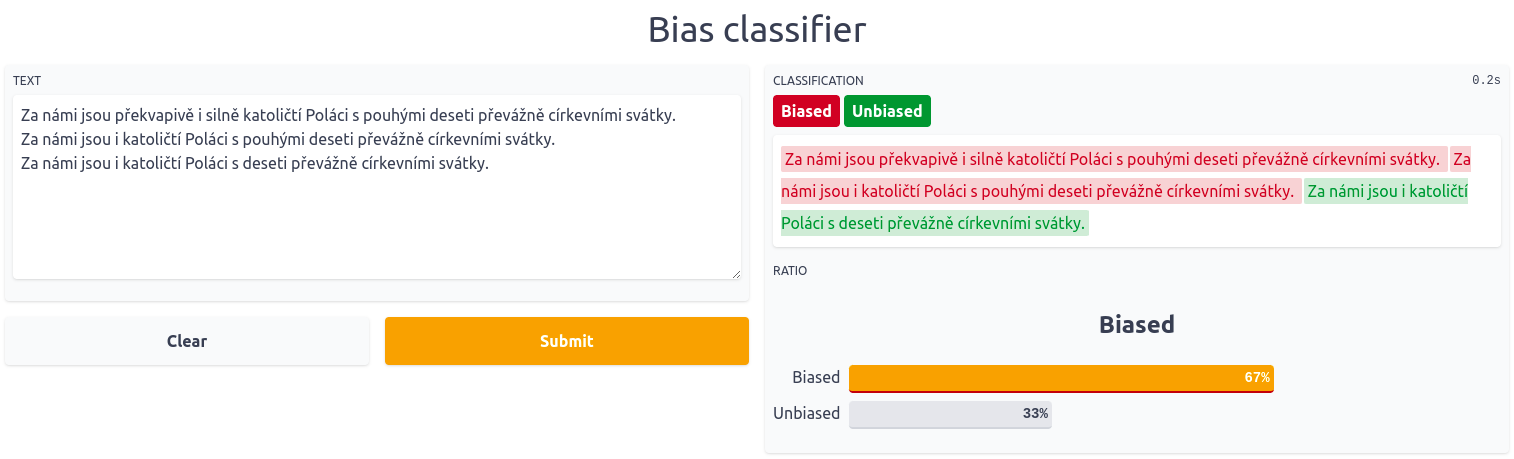
\includegraphics[scale=0.3]{my_modules/multimedia/bias.png}
  \caption{Example of the bias classifier demo usage. Red and blue color represent the biased and unbiased annotation respectively.}
  \label{fig:demodemo}
  }
\end{figure}
